\section{Voodiagramm}
\begin{figure}[ht]
    \centering
    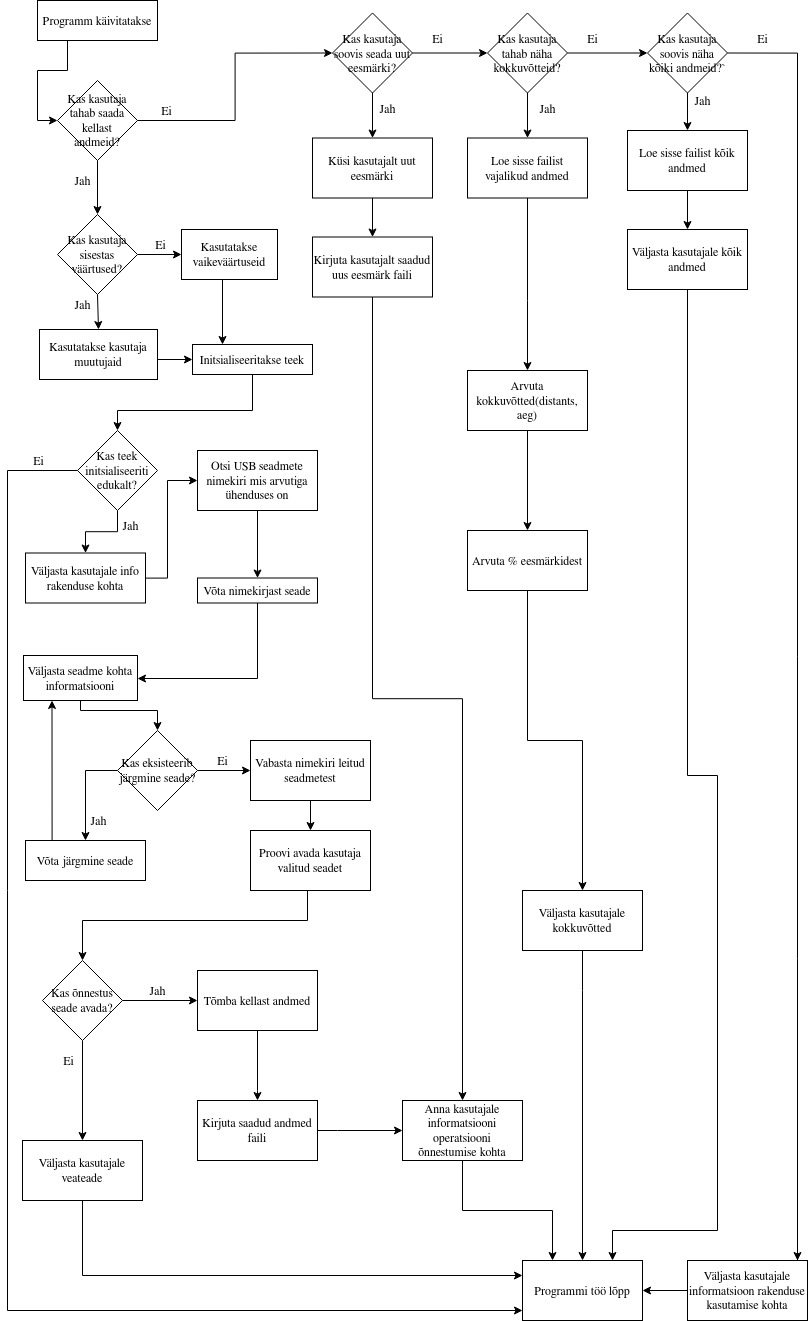
\includegraphics[width=.5\textwidth]{figures/flowchart.jpg}
    \caption{\textit{Voodiagramm programmi tööst}}
    \label{fig:flowchart}
\end{figure}


\section{Programmi töö}\label{sec:programmi-too}
Programmi alguses määratakse ära vaikeväärtused, mida rakendus saab kasutada.
Seejärel initsialiseeritakse \textit{libusb} teek ning antakse kasutajale teada mis versioon teegist kasutusel on.
Kui kasutaja on andnud rakendusele kaasa parameetrid, mille järgi soovib leida seadet, millega suhelda siis otsitakse seda konkreetset seadet ja kui kasutaja ei ole neid kaasa andnud, kastuatakse vaikeväärtuseid.
Kui otsitavat seadet ei leita, lõpetatakse programmi töö.
Kui otsitav seade on olemas ja ligipääsetav, siis programm jätkab seadme kohta informatsiooni väljastamisega.
Enne kellale päringute saatmist peab seadme avama, mida ka tehakse.
Kui avamine õnnestub, teatakse kasutajale, et see õnnestus, kui ei siis programmi töö katkestatakse.
Seejärel peaks hakkama kellast informatsiooni kättesaamine, kuid seda programmi osa projekti raames valmis ei saadud.

\section{Takistused}
